% !TeX spellcheck = de_DE
\documentclass{alex_gp}

\name{Alexander Helbok}
\course{Grundpraktikum}
\hwnumber{4}
\spacing{}

\begin{document}


\begin{mybox}{Laufzeitmessung}
	Ziel dieses Versuches ist es, die Schallgeschwindigkeit in der Luft mittels einer Laufzeitmessung zu bestimmen. Dazu wurde eine Lichtquelle (Taschenlampe) und das Messgerät auf einem Tisch positioniert und in einem Abstand von \( d = 3 \unit{m} \) vom IOLab wurde eine Markierung am Tisch vorgenommen. An diese Markierung wurde mit einem Brett der Lichtstrahl unterbrochen und gleichzeitig am Tisch ein lautes Geräusch erzeugt. Beide Signale kommen am IOLab an, wobei der Schlag vom Brett zeitlich leicht verzögert ankommt, da die Geschwindigkeit des Schalls wesentlich kleiner als die des Lichts ist. Aus dieser Zeitdifferenz lässt sich die Schallgeschwindigkeit berechnen. 
	
	Für die Distanz wurde ein Fehler von \( 1 \unit{cm} \) angenommen, um für den Ablesefehler, die Genauigkeit beim herunterschlagen der Brettes und die Positionierung des Sensors im IOLab zu kompensieren. Die Daten wurden bei einer Abfragerate von \( 2400 \unit{Hz} \) aufgezeichnet, weshalb die Unsicherheit in der Zeit auf \( 1/(2\cdot2400) \unit{1/Hz} = 0.21 \unit{µs} \) geschätzt wurde.
	
	\begin{figure}[H]	
		\centering
		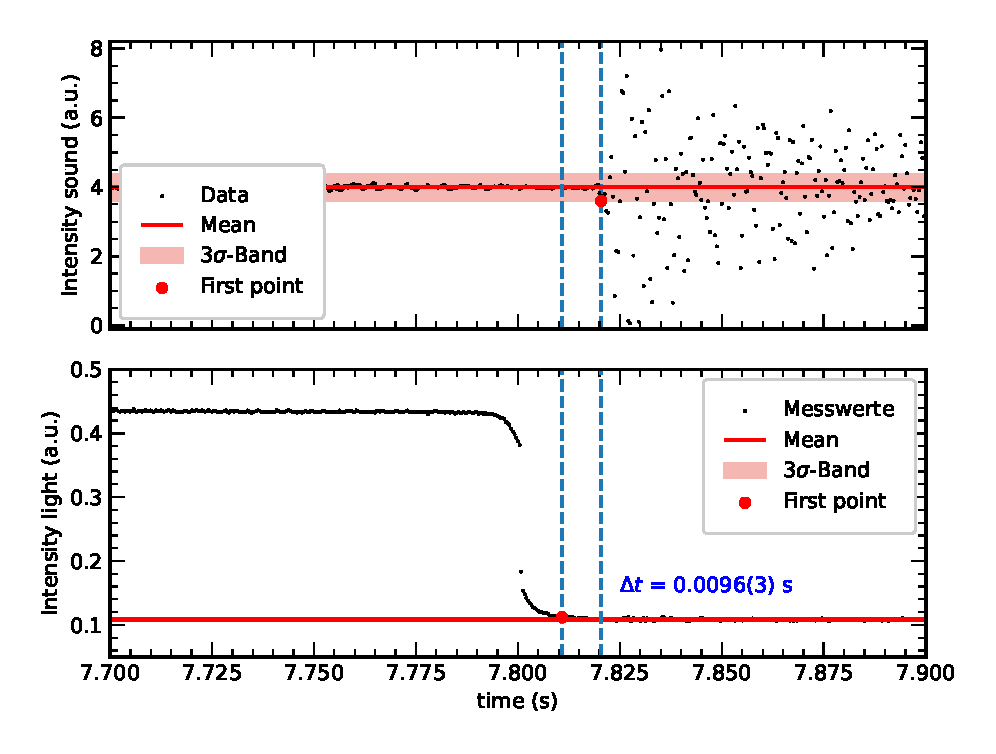
\includegraphics[width=\textwidth]{Versuch4_1.eps}
		\caption{Von oben nach unten sind Intensität des Schalls und des Lichts auf die Zeit aufgetragen. Die Daten werden ohne Fehlerbalken dargestellt, da diese zu klein wären. In Rot wurde der Mittelwert mit \( 3\sigma \)-Band aufgetragen und in blau ist die Zeitdifferenz zwischen den ersten beiden roten Punkten zu sehen.}
		\label{fig:laufzeit}
	\end{figure}

	Die Analyse der Daten ging wie folgt: es wurde zuerst der Mittelwert des Audiosignals vor dem Schlagereignis und der Mittelwert der Lichtintensität nach dem Schlagereignis berechnet. Das Audiosignal wird als registriert angenommen, wenn der erste Wert über \( 3\sigma \) vom Mittelwert abweicht, da die Wahrscheinlichkeit, dass dies durch Zufall eintrifft bei klein genug ist \( 0.3 \% \). Analog gilt das Lichtsignal als Unterbrochen sobald der erste Datenpunkt der Lichtmessung mehr also \( 3\sigma \) vom Mittelwert abweicht. 
	
	Die Zeitdifferenz \( \Delta t \) zwischen dem unterbrechen des Lichtstrahls und dem Ankommen der Schallwelle beim Messgerät berechnet sich aus 
	
	Damit berechnet sich die Schallgeschwindigkeit wie folgt
	\begin{equation}\label{eqn:v1}
		v = \frac{d}{\Delta t}
	\end{equation}
	
	In \autoref{fig:vmean} wurden die berechneten Geschwindigkeiten als normalisierte Gaußkurven auf die Geschwindigkeit aufgetragen. Hierbei sind 
	Die mittlere Gaußkurve ist dreimal 
	\begin{figure}[H]	
		\centering
		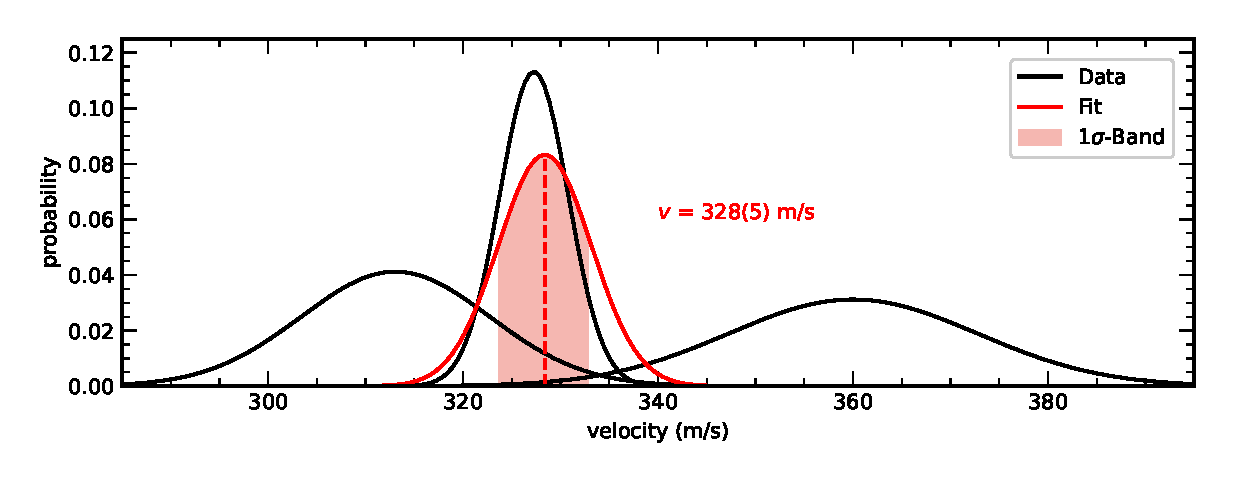
\includegraphics[width=\textwidth]{Versuch4_2.eps}
		\caption{Die gemessenen Geschwindigkeiten wurden als normalisierte Gaußkurven in schwarz auf die Geschwindigkeiten aufgetragen. In Rot der gewichtete Mittelwert, der sich als Überlagerung (und anschließende Normalisierung) der schwarzen Kurven ergibt. Das \( 1\sigma \) Intervall des Mittelwerts wurde farblich hinterlegt.}
		\label{fig:vmean}
	\end{figure}
\end{mybox}

\begin{mybox}{Resonanzmessung}
	Dafür wurde ein Kartonrohr der Länge \( L = 81.60(10) \unit{cm} \) und einem Durchmessen \( d = 0.40(10) \unit{cm} \) hergenommen. Ein Ende wurde mit dem IOLab abgedichtet und das Andere wurde offen gelassen und über Kopfhörer Töne reingespielt. Da das Rohr an einem Ende offen, muss man Korrekturen an der Länge vornehmen, sodass für die effektive Länge gilt \( L_{\text{eff}} = L + 0.6d = 81.84(12) \unit{cm} \).
	
	Die von den Lautsprechern erzeugten Schallwellen werden am geschlossenen Ende des Rohres reflektiert und interferieren mit den gegenläufigen Schwingungen. Bei bestimmten Frequenzen interferieren die Wellen maximal konstruktiv und kommt es zu stehenden Wellen. Aus der Schwingungsgleichung für Druckwellen kann man sich die Frequenzen ausrechnen, bei welchen stehende Wellen entstehen und man erhält
	\begin{equation}\label{key}
		f_n = (2n+1)\frac{c}{4L_{\text{eff}}}
	\end{equation}
    beziehungsweise für aufeinanderfolgende Frequenzen
    \begin{equation}\label{key}
    	f_{\text{n+1}} - f_{\text{n}} = \frac{c}{2L_{\text{eff}}}
    \end{equation}
\end{mybox}

\begin{mybox}{Berechnung der Schallgeschwindigkeit}
	Die Schallgeschwindigkeit lässt sich für ideale Gase mittels dem adiabatischen Kompressionsmodul berechnen 
	\begin{equation}\label{eqn:cad}
		c_{\text{ad}} = \sqrt{\gamma RT/M}
	\end{equation}
	wobei \( \gamma \approx 1.4 \) der Adiabatenindex, \( R = 8.3143 \unit{J K^{-1} mol^{-1}} \) die allgemeine Gaskonstante, \( T \) die Temperatur und \( M \approx 0.028973 \unit{kg/mol} \) die molare Masse des Gases beschreiben.
	Die Temperatur wurde mittel eines Thermometers auf \( 297(1) \unit{K} \) gemessen. 
	Setzt man nun Werte in \autoref{eqn:cad} ein, erhält man 
	\begin{equation}\label{eqn:cad2}
		c_{\text{ad}} = 345.45(6) \unit{\v}
	\end{equation}
	
	
	
	Der Adiabatenindex \( \gamma \), auch Wärmekapazitätsverhältnis genannt, wird durch das Verhältnis zwischen der Wärmekapazität eines Gases bei konstantem Druck zur Wärmekapazität bei konstantem Volumen beschrieben. 
	Für Luft gilt \( \gamma \approx 1.4 \) unter der Voraussetzung, dass der Luftdruck ungefähr bei \( 1 \unit{atm} \) und die Temperatur um \( 300 \unit{K} \) liegt.
	
	Aus \( 	\rho c \zeta_0 \omega = p_0 \) und \( \omega = 2\pi f \) folgt für \( \zeta_0 \) und \( v_0 \)
	\begin{align}\label{eqn:zeta}
		\zeta_0 &= \frac{p_0}{2\pi f\rho c} = 3.8394(6) \cdot 10^{-5} \unit{m} \\
		v_0 &= \zeta_0\omega = \frac{p_0}{2\rho c} = 0.24123(4) \unit{\v}
	\end{align}
	Substituiert man in der Zustandsgleichung für ideale Gase \( V = m/\rho \) erhält man für die Dichte
	\begin{equation}\label{eqn:density}
		\rho_0 = \frac{p_0M}{RT} = 0.01742 \unit{kg/m^3}
	\end{equation}
\end{mybox}

\end{document}